\documentclass{standalone}
\usepackage{tikz}
\usetikzlibrary{shapes,arrows.meta}
\begin{document}
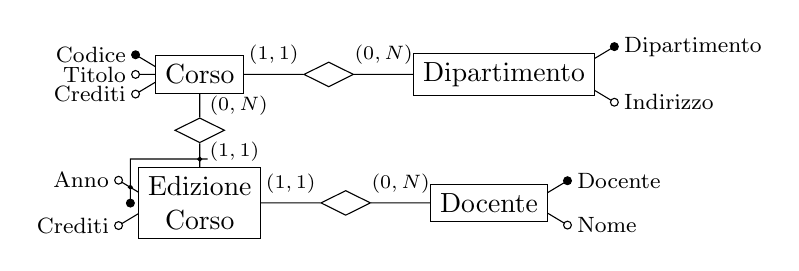
\begin{tikzpicture}
    \draw

    %%* Attributi:
    %%  node[draw, circle, inner sep=1pt, fill=black]{}node[right]{\footnotesize A}
    %%? Distanza orizzontale: E -(0.25,0.x)- A
    %%? Distanza verticale: E -(0,x * 0.22)- A

    %%* Cardinalità:
    %%  node[below right]{\scriptsize $(0,N)$}
    %%  node[above right]{\scriptsize $(0,N)$}
    %%  node[midway, above]{\scriptsize $(0,N)$}

    %%* Relazione:
    %%  node[draw, diamond, shape aspect=2, inner sep=3pt, anchor=90](r1){}
    %%  node[draw, diamond, shape aspect=2, inner sep=0.2pt, anchor=180](r2){R2}

    %%* Entità:
    %%  node[draw, rectangle, anchor=90](e1){}
    %%? Distanza verticale: E -(0.3)- R -(0.3) E
    %%? Distanza orizzontale: E -(0.75)- R -(0.75)- E

    %%* Corso 
    (0,0)node[draw, rectangle, anchor=90](cds){Corso}
    (cds.170)--++(-0.25,0.15)node[draw, circle, inner sep=1pt, fill=black]{}node[left]{\footnotesize Codice}
    (cds.180)--++(-0.25,0)node[draw, circle, inner sep=1pt, fill=white]{}node[left]{\footnotesize Titolo}
    (cds.190)--++(-0.25,-0.15)node[draw, circle, inner sep=1pt, fill=white]{}node[left]{\footnotesize Crediti}

    %%* Dipartimento
    (cds.0)--++(0.75,0)node[midway, above]{\scriptsize $(1,1)$}node[draw, diamond, shape aspect=2, inner sep=3pt, anchor=180](r1){}
    (r1.0)--++(0.75,0)node[midway, above]{\scriptsize $(0,N)$}node[draw, rectangle, anchor=180](dip){Dipartimento}
    (dip.10)--++(0.25,0.15)node[draw, circle, inner sep=1pt, fill=black]{}node[right]{\footnotesize Dipartimento}
    (dip.350)--++(0.25,-0.15)node[draw, circle, inner sep=1pt, fill=white]{}node[right]{\footnotesize Indirizzo}

    %%* Edizione Corso
    (cds.270)--++(0,-0.3)node[midway, right]{\scriptsize $(0,N)$}node[draw, diamond, shape aspect=2, inner sep=3pt, anchor=90](r2){}
    (r2.270)--++(0,-0.2)node[midway, right]{\scriptsize $(1,1)$}node[draw, circle, inner sep=0.5pt, fill=black](a){}--++(0,-0.1)node[draw, rectangle, anchor=90, align=center](ed){Edizione\\Corso}
    (ed.170)--++(-0.1,0.06)node[draw, circle, inner sep=0.5pt, fill=black](b){}--++(-0.15,0.09)node[draw, circle, inner sep=1pt, fill=white]{}node[left]{\footnotesize Anno}
    (ed.190)--++(-0.25,-0.15)node[draw, circle, inner sep=1pt, fill=white]{}node[left]{\footnotesize Crediti}
    
    (a)++(0.1,0)-|(b)--++(0,-0.2)node[draw, circle, inner sep=1pt, fill=black]{}

    %%* Docente
    (ed.0)--++(0.75,0)node[midway, above]{\scriptsize $(1,1)$}node[draw, diamond, shape aspect=2, inner sep=3pt, anchor=180](r3){}
    (r3.0)--++(0.75,0)node[midway, above]{\scriptsize $(0,N)$}node[draw, rectangle, anchor=180](doc){Docente}
    (doc.10)--++(0.25,0.15)node[draw, circle, inner sep=1pt, fill=black]{}node[right]{\footnotesize Docente}
    (doc.350)--++(0.25,-0.15)node[draw, circle, inner sep=1pt, fill=white]{}node[right]{\footnotesize Nome}

    ;
\end{tikzpicture}
\end{document}